\documentclass[12pt]{article}
\usepackage{graphicx}
\usepackage{amsmath}

\begin{document}
CSCI-4100 Assignment 6\\
Yichuan Wang \\
RIN:661414395\\\\

EXERCISES\\
3.4\\%part e only...
(a) We are given $y=Xw^*+\epsilon$, and by definition $\hat{y}=Hy$. We therefore have: 
$$\hat{y}=Hy=X(X^TX)^{-1}X^T(Xw^*+\epsilon)=X(X^TX)^{-1}X^TXw^*+H\epsilon=Xw^*+H\epsilon$$
(b) $\hat{y}-y=Xw^*+H\epsilon-(Xw^*+\epsilon)=(H-I)\epsilon$ The matrix is therefore $$H-I$$
(c) $$E_{in}(w_{lin})=\frac{1}{N}\parallel\hat{y}-y\parallel^2=\epsilon^T(H-I)^T(H-I)\epsilon$$
Since $H-I$ is symmetric, we have $(H-I)^T=H-I$, and therefore $(H-I)^T(H-I)=(H-I)^2=(I-H)^2=I-H$
	$$E_{in}(w_{lin})=\frac{1}{N}\epsilon^T(I-H)^2\epsilon=\frac{1}{N}\epsilon^T(I-H)\epsilon$$
(d) $$E_D[E_{in}(w_{lin})] = E_D[\frac{1}{N}\epsilon^T(I-H)\epsilon]=\frac{1}{N}(E_D[\epsilon^T\epsilon]-E_D[\epsilon^TH\epsilon])$$
	We know that $E_D[\epsilon^T\epsilon] = N\sigma^2$, so we have
	$$E_D[E_{in}(w_{lin})] = E_D[\frac{1}{N}\epsilon^T(I-H)\epsilon]=\sigma^2-\frac{1}{N}E_D[\epsilon^TH\epsilon]$$
	We know that $$\epsilon^TH\epsilon = \sum_{i=1}^N\sum_{j=1}^NH_{ij}\epsilon_i\epsilon_j=\sum_{i=1}^NH_{ii}\epsilon_i^2+\sum_{i=1}^N\sum_{j=1,i \neq j}^NH_{ij}\epsilon_i\epsilon_j=trace(H)\epsilon_i^2+\sum_{i=1}^N\sum_{j=1,i \neq j}^NH_{ij}\epsilon_i\epsilon_j$$   
	By definition we have $E_D[\epsilon^2]=\sigma^2$ ,$E_D[\epsilon_i\epsilon_j]=E_D[\epsilon_i]E_D[\epsilon_j]=0$, and we are given that $\epsilon$ is independently generated for each data point. And from exercise 3.3 we know that $trace(H)=d+1$. So we have $$E_D[\epsilon^TH\epsilon]=(d+1)\sigma^2$$
And therefore we have
$$E_D[E_{in}(w_{lin})]=\sigma^2+\frac{1}{N}(d+1)\sigma^2=\sigma^2(1-\frac{d+1}{N})$$
PROBLEMS\\
(e) The proof is as following:\\
$$E_{TEST}(w_{lin})=\frac{1}{N}(H\epsilon-\epsilon')^T(H\epsilon-\epsilon')$$
$$E_{TEST}(w_{lin})=\frac{1}{N}(\epsilon^TH^T-\epsilon'^T)(H\epsilon-\epsilon')$$
$$E_{TEST}(w_{lin})=\frac{1}{N}(\epsilon^TH^TH\epsilon-\epsilon^TH^T\epsilon'-\epsilon'^TH\epsilon+\epsilon'^T\epsilon')$$
$$E_{TEST}(w_{lin})=\frac{1}{N}(\epsilon^TH\epsilon-\epsilon^TH^T\epsilon'-\epsilon'^TH\epsilon+\epsilon'^T\epsilon')$$
It is observed that there are four terms in the parentheses; we take these four terms from left to right  and label the expected version of them as $T1$,$T2$,$T3$, and $T4$.
We have the following:
$$T1=E[\epsilon^TH\epsilon]$$
$$T2=E[-\epsilon^TH^T\epsilon']$$
$$T3=E[-\epsilon'^TH\epsilon]$$
$$T4=E[\epsilon'^T\epsilon']$$
Now we analyse these four terms one by one:\\
For T1:
This term is same as the term that appeared in part(d); we sum up the trace term and zero the non-trace term. Please refer to detailed calculation for the term $E[\epsilon^TH\epsilon]$ in part(d) of this problem. The result is as following:
$$T1=(d+1)\sigma^2$$
For T3:
$$T3=E[-\epsilon'^TH\epsilon]=E[\sum_i\sum_jH_{ij}\epsilon_i\epsilon_j]=\sum_i\sum_jH_{ij}E[\epsilon_i]E[\epsilon_j]$$
Since $\epsilon$ and $\epsilon'$ are independent and both have zero mean, every term in this sum has expected value zero, and thus this term is zero:
$$T3=0$$
Same thing applies for T2 (as for T3 in the former derivation):
$$T2=E[-\epsilon^TH^T\epsilon']=0$$
For T4:
$$T4=E[\epsilon^TH\epsilon]=N\sigma^2$$
We know the above result for T4 since $\epsilon$ and $\epsilon'$ share the same mean and variance.\\

Now sum up the non-zero terms and get the expression for $E_{TEST}(w_{lin})$:
$$E_{TEST}(w_{lin})=\frac{1}{N}(T1+T2+T3+T4)=\frac{1}{N}(T1+T4)=\frac{1}{N}(N\sigma^2+(d+1)\sigma^2)=(1+\frac{d+1}{N})\sigma^2$$
\\\\\\\\\\\\\\\\\\\\\\\\\\\\\\\\\\\\\\\\\\\\\\\\\\\\\\\\
PROBLEMS
3.1\\%DONE
(a)\\
The perceptron result is as following:
\\$w0=-1602$, $w1=-38.94$, $w2=138.44$\\
The perceptron image is as following:\\
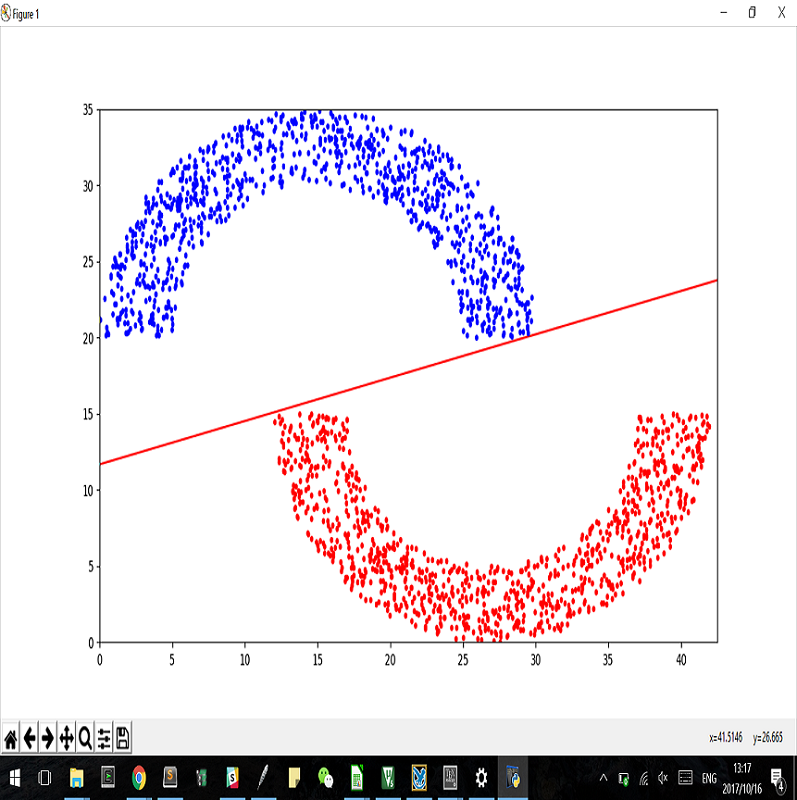
\includegraphics[scale=0.8]{3-1a}\\
(b)\\
The linear regression result is as following:\\
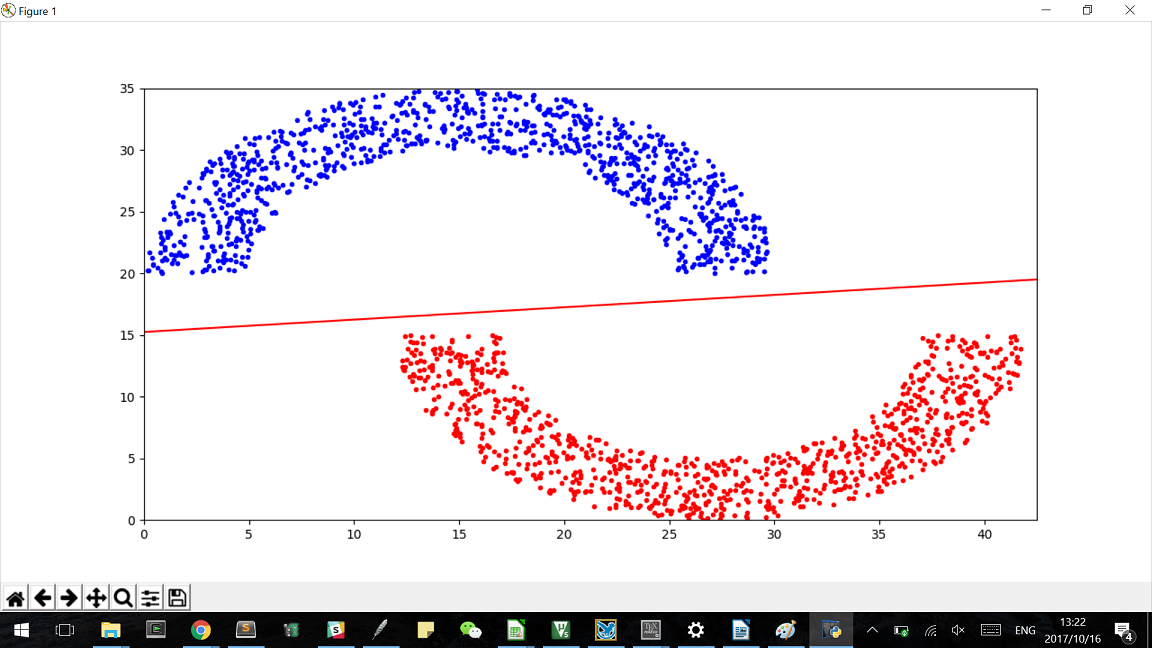
\includegraphics[scale=0.6]{3-1b}\\
The linear regression result $w_{lin}$ is:\\ $w0=-1.223$, $w1=-0.008$, $w2=0.0789$\\
The perceptron starting from $w_{lin}$ converges at the first iteration since the data is already separated with linear regression.\\

3.2\\%DONE
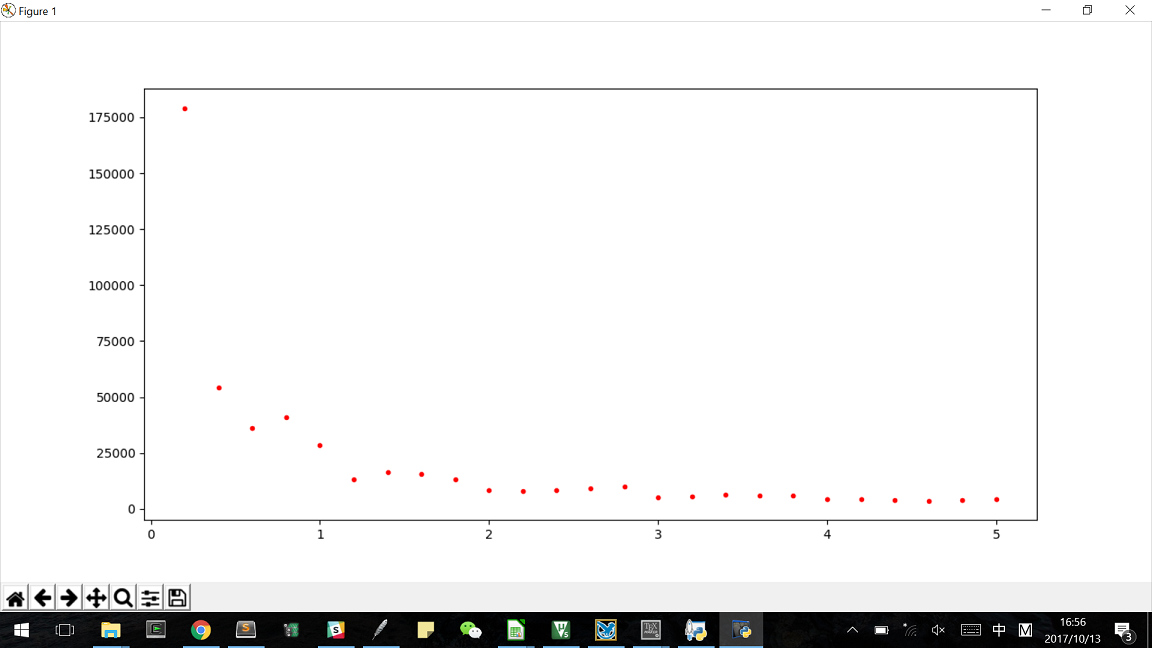
\includegraphics[scale=0.6]{3-2}\\
The result is shown for averaging 10 rounds of experiment results for each $sep$. X-axis is $sep$, and y-axis is number of iterations. The observation is that the converging step number $t$ decreases as $sep$ increases. According to Problem 1.3, the upper bound of converging step number $t$ is inversely proportional to the square of the smallest $w^Tx$ of $w*$ (a $w$ that separates the data). Even though no clear algebraic relationship is shown from this experiment, the weak inverse relationship between $sep$ and converging step number $t$ is pointing towards the same direction as problem 1.3 does.

3.6\\
(a) Having all $w^Tx>0$ implies having $w^Tx\geq 1$; we can simply take a $w$ that separates the data and scale it up until all the $w^Tx$ becomes larger or equal to 1.\\\\
(b) The optimization variable $z$ is the weight vector $w$. Linear programming can be divided into standard maximum problem and standard minimum problem, and here we are dealing with the standard minimum problem. Problem part(a) has already gave us the constraint, so $A$ is therefore a $n*(d+1)$ matrix such that each row is $y_nx_n$. $b$ is simply a $n\times 1$ vector of 1. In this case we don't really care about $c$ since all we need is to satisfy the constraints, and $c$ can be anything we want, just to get the algorithm going. \\

3.8\\%DONE
	The derivation is as following:
	$$E_{out}=E[(h(x)-y)^2]=\int_x\int_y(h(x)-y)^2p(x)p(y|x)dydx$$
	$$E_{out}=\int_x\int_y(h(x)^2-2h(x)+y^2)p(x)p(y|x)dydx$$
	$$E_{out}=\int_xh(x)^2p(x)\int_yp(y|x)dydx-2\int_xh(x)p(x)\int_yyp(y|x)dydx+\int_xp(x)\int_yy^2p(y|x)dydx$$
	By definition we have $\int_yy^2p(y|x)dy=E[y^2|x]=E[y|x]^2+VAR[y|x]$,$\int_yyp(y|x)dy=E[y|x]$ and $\int_yp(y|x)dy=1$
	So we have
	$$E_{out}=\int_xh(x)^2-2h(x)E[y|x]+(E[y|x])^2+VAR[y|x]p(x)dx$$
	$$E_{out}=\int_x(h(x)-E[y|x])^2p(x)+VAR[y|x]p(x)dx$$
	$$E_{out}=\int_x(h(x)-E[y|x])^2p(x)dx+\int_xVAR[y|x]p(x)dx$$
	Since the term $\int_xVAR[y|x]p(x)dx$ is $E[VAR[y|x]]$, it is a constant. So what we can do to minimize $E_{out}$ is to make this term as small as possible:$$\int_x(h(x)-E[y|x])^2p(x)dx$$ which yields $h(x)=E[y|x]$ and $h(x)-E[y|x]=0$\\
	To show that $E[\epsilon(x)]=0$, we do the following:
	$$y(x)=h*(x)+\epsilon(x)$$
	$$E[y(x)]=E[y|x]=E[h*(x)+\epsilon(x)]=E[h*(x)]+E[\epsilon(x)]$$
	$$E[y|x]=h*(x)=E[y|x]=E[E[y|x]]=E[h*(x)]$$
	$$E[h*(x)]=E[h*(x)]+E[\epsilon(x)]$$
	$$E[\epsilon(x)]=0$$

HAND WRITTEN DIGITS\\%DONE
(a) Plottings(1 and 5)\\
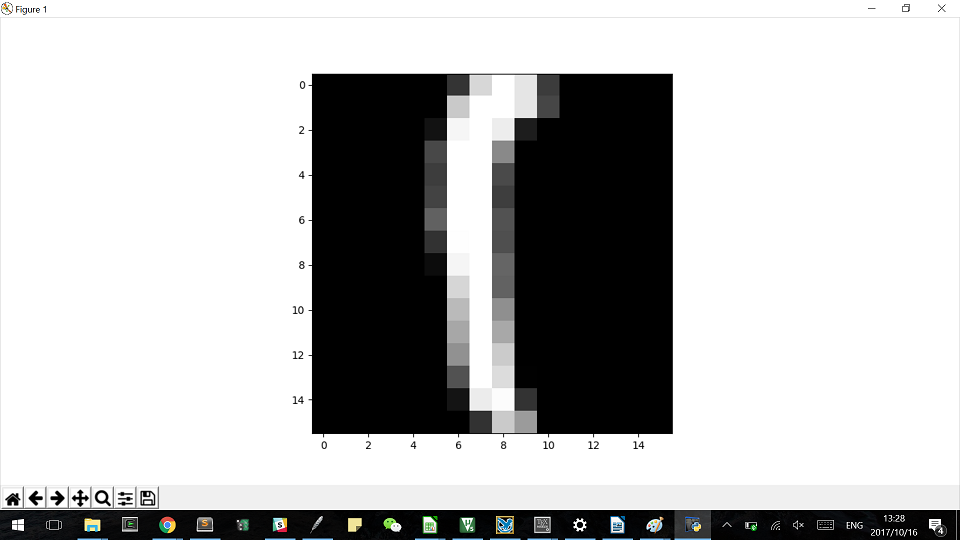
\includegraphics[scale=0.8]{1}\\
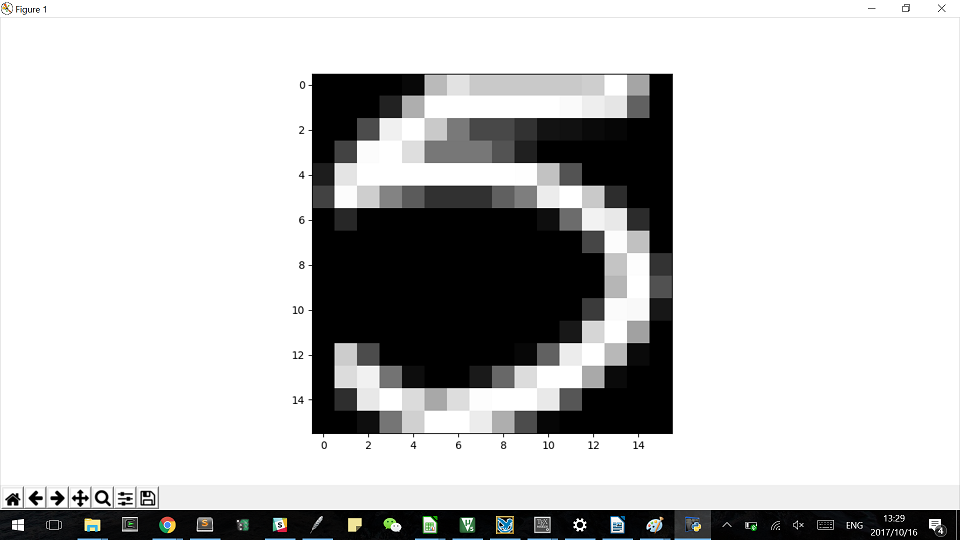
\includegraphics[scale=0.8]{5}\\
(b) I used two features: Feature 1 is the left-right asymmetry, and feature 2 is up-down asymmetry. 
The left-right asymmetry is defined as the absolute difference between an image and its vertical-axis flipped version, and the up-down asymmetry is defined as the absolute difference between an image and its horizontal-axis flipped version.\\
Math definition for feature 1:\\
$$\sum_{i=0}^{15}\sum_{j=0}^7|pix[i][j]-pix[i][15-j]|$$
Math definition for feature 2:\\
$$\sum_{i=0}^7\sum_{j=0}^{15}|pix[i][j]-pix[15-i][j]|$$
(c)\\
For both images, x-axis is feature 1, and y-axis is feature 2.\\
training data result:\\
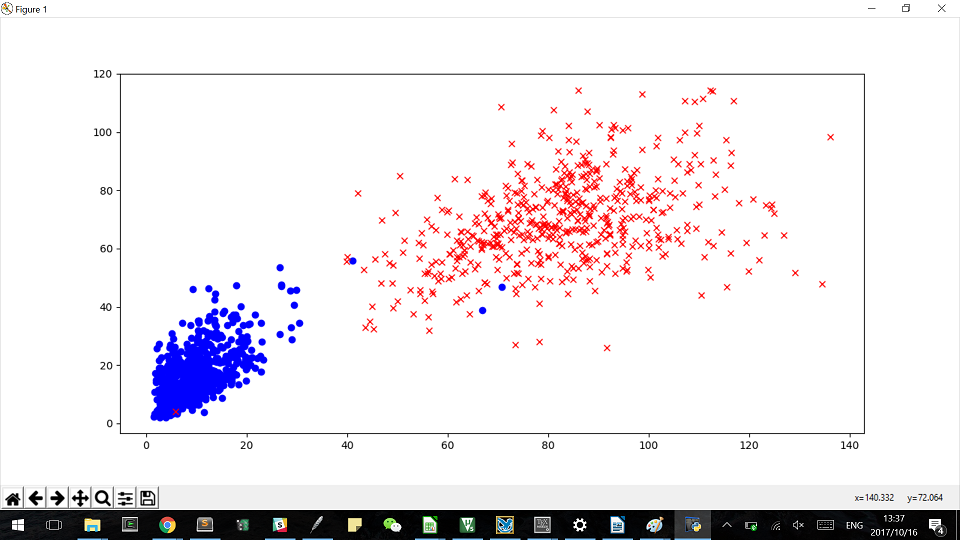
\includegraphics[scale=0.8]{train1_5}\\
testing data result:\\
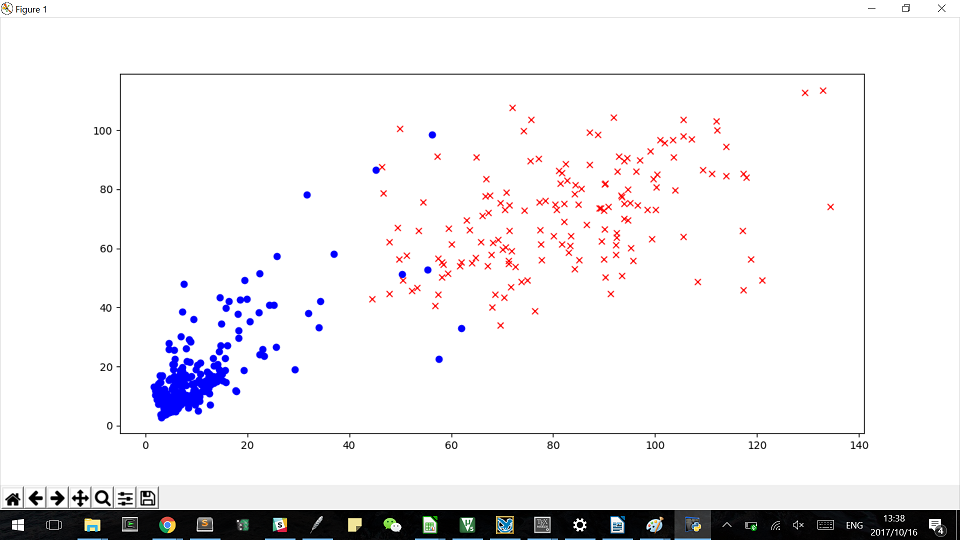
\includegraphics[scale=0.8]{test1_5}\\
\end{document}












